This section will cover the configuration of the various servers on your platform. 
\subsubsection{Minimum Software Requirements}
To run the service you are required to have \href{https://git-scm.com}{git}, \href{https://nodejs.org}{NodeJS} v6 or higher (Which comes with \href{https://www.npmjs.com}{npm} v3 or higher), \href{https://www.rabbitmq.com/download.html}{RabbitMQ}, \href{https://www.mongodb.com/download-center?jmp=nav#community}{MongoDB} and \href{http://rethinkdb.com/docs/install}{RethinkDB} installed on your platform.
\subsubsection{Configuration}
	\begin{enumerate}
		\item \textbf{Download Source Code} \\
		The source code is located on \href{https://github.com}{Github} at the : \url{https://github.com/Coeus2016/geospatial-data-processor-and-visualizer}. You are required to clone the repository. There are two ways to clone the repository:\\
		\begin{itemize}
			\item By using the git command line. In the root folder run the following commands
			\begin{verbatim}
			$git clone https://github.com/Coeus2016/geospatial-data-processor-and
			-visualizer.git		
			\end{verbatim}
		
		\item By downloading the a *zip file from this url \url{https://github.com/Coeus2016/geospatial-data-processor-and-visualizer}\\
		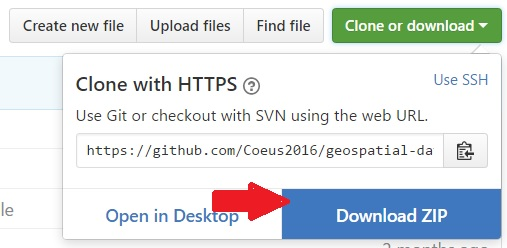
\includegraphics[width=\textwidth]{clone} \\[0.5cm]
		
		\end{itemize}
		
		\item \textbf{Installing Required Modules}\\
		Now that you have downloaded the repository, navigate to the root folder and perform the following commands.
		\begin{verbatim}
			$git submodule update --init --recursive
			$npm install			
			\end{verbatim}
			These commands updated the submodules and install the node modules required to run the server	
	\end{enumerate}

\subsubsection{Starting The Service}
Once you have downloaded and installed all required modules, you are ready to start the service. The following steps need to be followed to insure a safe start of the system.
\begin{enumerate}
	\item Before you can start the application server, you need to make sure all other used services (RethinkDB, MongoDB, RabbitMQ) have been started\footnote{A lot of the time they are configured to start when the computer is booted otherwise you are required to start the services manually in different terminal windows.}. 
	\item Once the other services have been started, running the following command will start the application. 
	\begin{verbatim}
		$npm start			
	\end{verbatim}
	The backend Server will run on port 3200, the scrapper on port 3500 and the webserver on port 3000. To view the website, simply visit \url{http://localhost:3000} on your browser.
\end{enumerate}